\section{Background Study}
 There are different type of anomalies that can be mapped with different types of attacks~\cite{ahmed2016survey}. The main attacks are DoS, Probe, U2R and R2U attack.

The differnt types of anomalies are as follows:
\begin{itemize}
    \item \textbf{Point anomaly}:Rather than on the whole dataset, point anomaly occurs on a specific data instance.
    \item \textbf{Contextual anomaly}: When data instances are anomalous in a specific context, that can be called contextual anomaly. Like during season of festivities, credit card transactions are higher than regular. But it is not the same case for a non-festive season. High expenditure in a non-festive season can be pointed as a contextual anomaly. Occurrence of contextual anomalies depends on the availability of context attributes in the data. ~\cite{chandola2009anomaly}.
    \item \textbf{Collective anomaly}: When a collection of similar kind of data instances act anomalously with respect to the whole dataset, then it can be deemed as collective anomaly~\cite{ahmed2016survey}.
    
\end{itemize}

\begin{figure}[tb]
  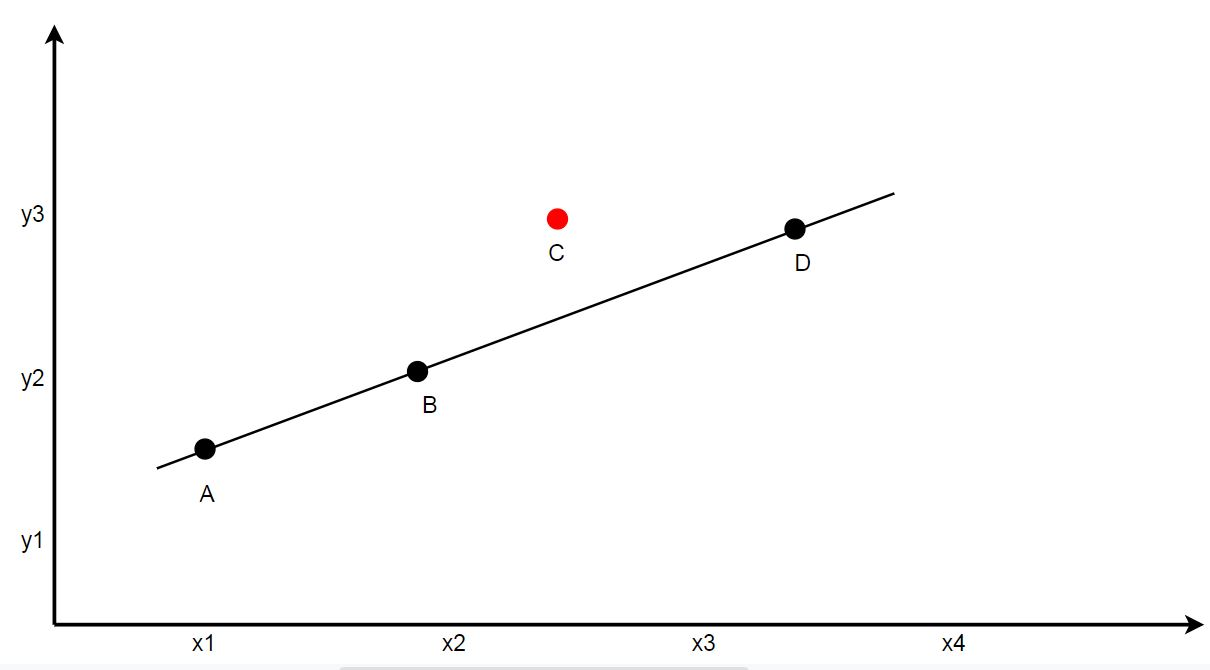
\includegraphics[width=\linewidth]{point.JPG}
  \caption{C is showing point anomaly.}
  \label{fig:point}
\end{figure}

\begin{figure}[bth]
  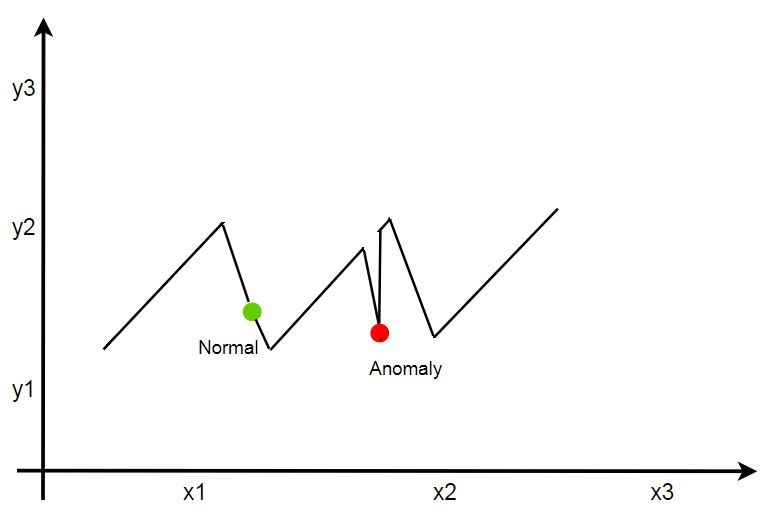
\includegraphics[width=\linewidth]{contextual.JPG}
  \caption{Contextual anomaly.}
  \label{fig:point}
\end{figure}

\begin{figure}[h]
  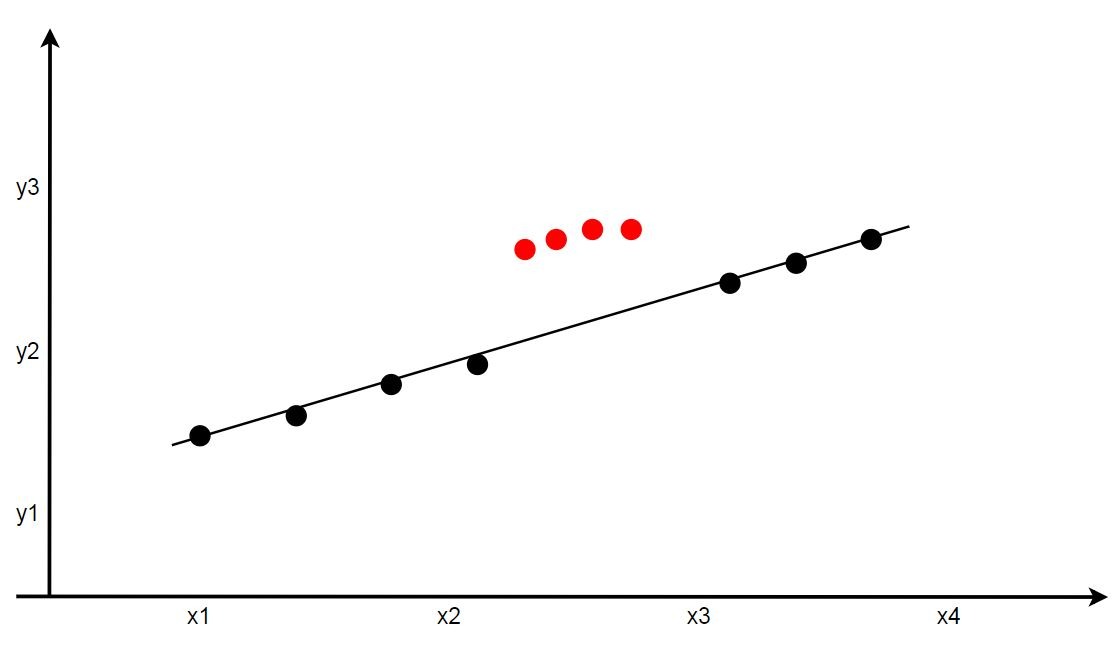
\includegraphics[width=\linewidth]{collective.JPG}
  \caption{4 red points are collectively showing anomaly.}
  \label{fig:point}
\end{figure}

There are different types of  attacks as follows:

\begin{itemize}
    \item \textbf{DoS attack}: DoS or Denial of Service represents the type of attack where the attacker makes a machine or resource unavailable to the legit users by blocking it intentionally through flooding. This attack keeps the memory resources of the server full so that legitimate user requests can not get through. Therefore, the user requests are denied.
    \item \textbf{Probe attack}: This type of attack is used to gather information about a targeted network or host and, more formally, for reconnaissance purposes ~\cite{ahmed2016survey}. This is used to know about the number \& type of machines connected in the network \& to know about installed softwares in the host machine. This is the step before an actual attack.
    \item \textbf{User to Root (U2R)}: When attacker wants to gain illegal access to an administrative account, U2R attack is used. Attacker can use social engineering approach or password sniffing \& being successful on those efforts, can access a normal user account. After gaining access in normal account \& exploiting vulnerabilities, attacker can gain the privilege of a super user.
    \item \textbf{Remote to User (R2U)}: It is launched when an attacker wants to gain local access as a user of a targeted machine to have the privilege of sending packets over its network (also known as R2L) ~\cite{ahmed2016survey}. Normally the attacker uses a trial and error method to guess the password. In some sophisticated attacks, attacker installs a sniffing tool to capture the password before going through the system.
\end{itemize}

Ahmed et al. ~\cite{ahmed2016survey} mapped the point anomaly with the U2R \& the R2U attacks. These type of attacks are condition specific and are hard to launch compared to other attacks. They mapped DoS attack to collective anomaly ~\cite{ahmed2014network} and Probe attack to contextual anomaly. DoS attack is specified by the collective attack of same nature. That is why it is mapped to collective anomaly as numerous connection requests are sent to deliver this attack. As probing is done on specific intention of gathering information, it is mapped with contextual anomaly.

\begin{figure}[b]
  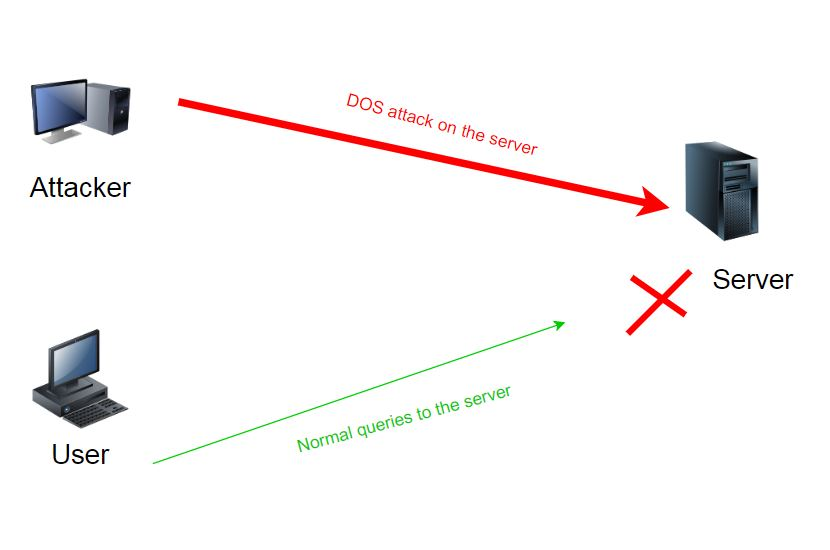
\includegraphics[width=\linewidth]{DOS2.JPG}
  \caption{DOS attack.}
  \label{fig:DOS}
\end{figure}


